\section{\texorpdfstring{SUBGROUPS AND QUOTIENT GROUPS OF \(\mathbf{R}^n\)}{SUBGROUPS AND QUOTIENT GROUPS OF R TO THE N}}

Let us first introduce the following convention: if G is a topological group, we have defined (Chapter III, § 2) the product group \(G^{n}\) of n factors equal to G, for each integer n \textgreater{} 0. In this section, we shall extend this definition to the case n = 0 by the convention that \(G^{0}\) denotes a group consisting of only one element. If H is any group, we shall identify \(G^{0} \times H\) with H.

\pandocbounded{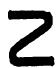
\includegraphics[keepaspectratio]{images/part001_b5dea1c7.jpg}}

On the set \(\mathbf{R}^n\) , we shall have to consider on the one hand its (additive) topological group structure and on the other hand its vector space structure over the field \(\mathbf{R}\) (Chapter VI, § 1, no. 3). Given a subset \(\mathbf{A}\) of \(\mathbf{R}^n\) , we may envisage the subgroup of \(\mathbf{R}^n\) generated by \(\mathbf{A}\) (the set of all linear combinations of points of \(\mathbf{A}\) , with integer coefficients) and also the vector subspace generated by \(\mathbf{A}\) (the set of all linear combinations of points of \(\mathbf{A}\) , with real coefficients); these two notions must be carefully distinguished. In accordance with the definitions made in algebra, the rank of \(\mathbf{A}\) is the dimension of the vector subspace \(\mathbf{V}\) of \(\mathbf{R}^n\) generated by \(\mathbf{A}\) ; to say that \(\mathbf{A}\) is of rank \(p\) is therefore equivalent to saying that there are \(p\) points \(x_i \in \mathbf{A}\) which form a free system with respect to the field \(\mathbf{R}\) (in other words, the relation \(\sum_{i} t_i x_i = 0\) , where the \(t_i\) are real, implies \(t_i = 0\) for each \(i\) ) and form a basis of \(\mathbf{V}\) (which means that every point of \(\mathbf{V}\) is a linear combination of the \(x_i\) with real coefficients).

In what follows we shall also have to make use of the notion of a system of points of \(\mathbf{R}^n\) which are free with respect to the field \(\mathbf{Q}\) of rational numbers; such a system is a finite subset \((\pmb{x}_i)\) of \(\mathbf{R}^n\) such that the relation \(\sum_{i} r_i x_i = 0\) , where the \(r_i\) are rational numbers (or integers --- it comes to the same thing), implies that \(r_{i}=0\) for each i. This notion must be carefully distinguished from that of a free system with respect to R: every system which is free with respect to R is free with respect to Q, but the converse is false (for example, the numbers 1 and \(\sqrt{2}\) in R form a free system with respect to Q, but not a free system with respect to R). Whenever we speak of a free system without qualification, we shall always mean a free system with respect to R. It is therefore necessary to distinguish on \(R^{n}\) the vector space structure with respect to R from the vector space structure with respect to Q; in particular, the vector subspace with respect to Q generated by a subset A of \(R^{n}\) is the set U of all linear combinations of A with rational coefficients; it is contained in the vector subspace V (with respect to R) generated by A, but is in general distinct from V. The dimension of U (with respect to Q) is called the rational rank of A; it is at least equal to the rank of A defined above (the dimension of V with respect to R); it may be infinite if A is an infinite set, while the rank of any non-empty subset of \(R^{n}\) is always \(\leqslant n\) ; in particular, the rational rank of any uncountable subset of \(R^{n}\) is always infinite, because any finite-dimensional vector space over Q is countable.

\pandocbounded{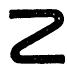
\includegraphics[keepaspectratio]{images/part001_3371d17f.jpg}}

In this section we shall first determine the structure of the closed subgroups of the additive group \(R^{n}\) .

